% File: diary.tex
% Date: Sun Jun 23 16:20:06 2013 +0800
% Author: Yuxin Wu <ppwwyyxxc@gmail.com>
\section{过程记录}
本项目的开发记录可以通过git查看. 项目托管在github\footnote{\url{https://github.com/ppwwyyxx/Ray-Tracing-Engine}}
及计算机系git9\footnote{\url{http://git.net9.org/ppwwyyxx/ray}}上,并于6月24日开源.

\begin{enumerate}
  \item
    首次出现正常的图片. 用了一个$ x-y$平面上的无限大平面及一个点光源。
    此时仅仅参考\cite{phong}考虑了基本Phong模型中的漫反射与环境光,已经可以看到左下部分亮度较高,符合预期。

    另外,远处的黑白纹理误差较大,不知是不可改进的浮点误差还是我的处理有误。
    \begin{figure}[H]
      \centering
      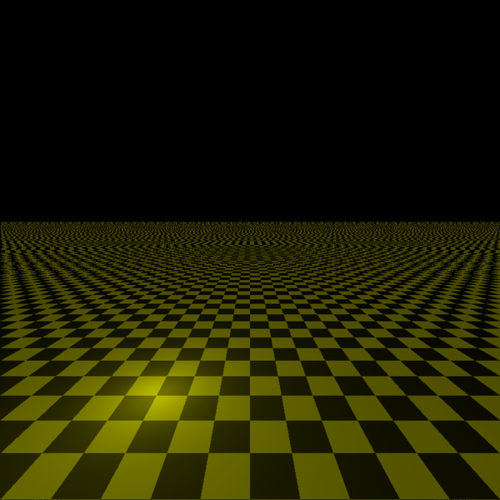
\includegraphics[scale=0.4]{img/first_pic.png}
      \caption{\label{fig:first}}
    \end{figure}

  \item
    依照Beer-Lambert定律\cite{beer}对光线能量进行了按距离的减弱:
    \[ E = E_0 e^{distance * density}\]
    使得远处的纹理更自然.
    \begin{figure}[H]
      \centering
      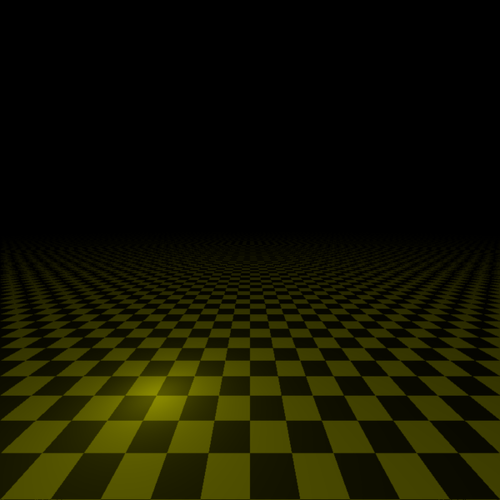
\includegraphics[scale=0.4]{img/plane_with_beer.png}
      \caption{Beer-Lambert定律效果图\label{fig:beer}}
    \end{figure}

  \item

    考虑了Phong模型中的高光,并对$ x-y$平面和$ y-z$平面加入了反射系数,有了互相反射的效果,并且
    左下部分能够看到高光.打开\verb|-O3|编译开关时,在我的机器上渲染一张$600 \times 600$的图片需要0.39s.
    \begin{figure}[H]
      \centering
      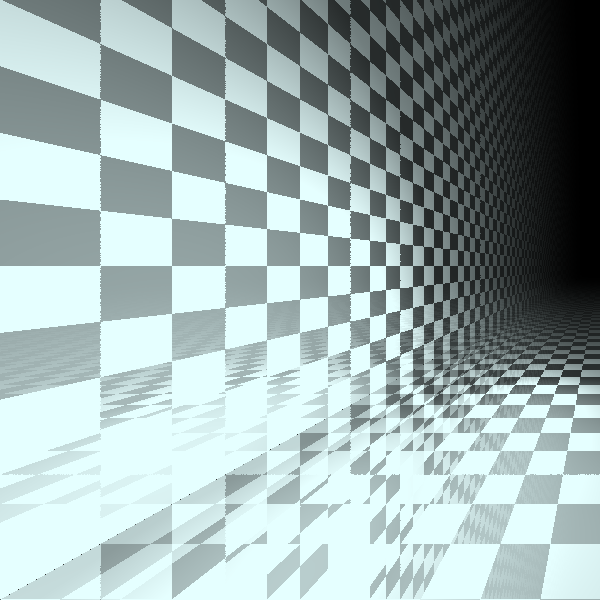
\includegraphics[scale=0.4]{img/specular.png}
      \caption*{\label{fig:specular}}
    \end{figure}

  \item

    使用球模型,可以看到明显的高光效果。同时由于球面\verb|specular|参数高,使得球下部反射了平面。
    \begin{figure}[H]
      \centering
      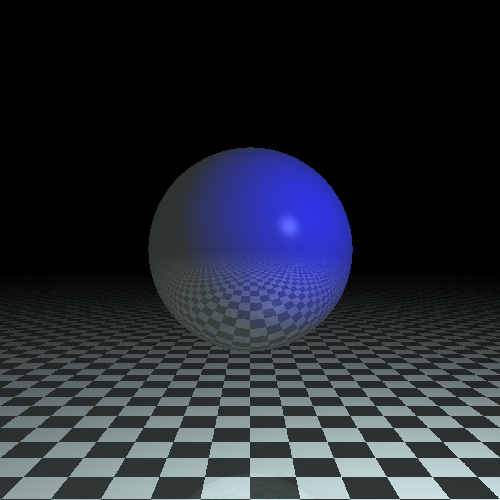
\includegraphics[scale=0.4]{img/ball.png}
      \caption*{\label{fig:ball}}
    \end{figure}

  \item
    对于找到的交点,判断它与光源之间是否被挡住,若被挡住就不计算漫反射和高光. 这样实现了阴影效果.
    \begin{figure}[H]
      \centering
      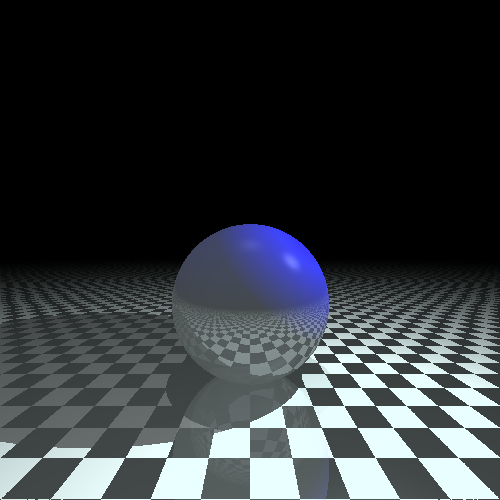
\includegraphics[scale=0.4]{img/shadow.png}
      \caption*{\label{fig:shadow}}
    \end{figure}

  \item 对根据视点及对象生成视图(View)的方案进行修改,以支持视图的旋转,缩放.并利用opencv的key event实现了gui的旋转,缩放控制.
    \begin{figure}[H]
      \centering
      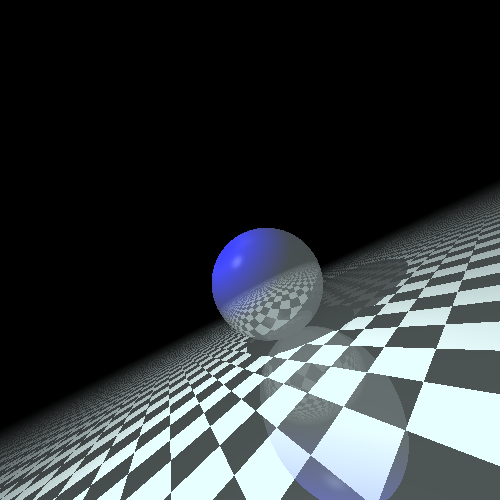
\includegraphics[scale=0.4]{img/rotate.png}
      \caption*{\label{fig:rotate}}
    \end{figure}

  \item 加入了透射功能,依照预定义的介质密度及折射定律计算出射光方向.
    \begin{figure}[H]
      \centering
      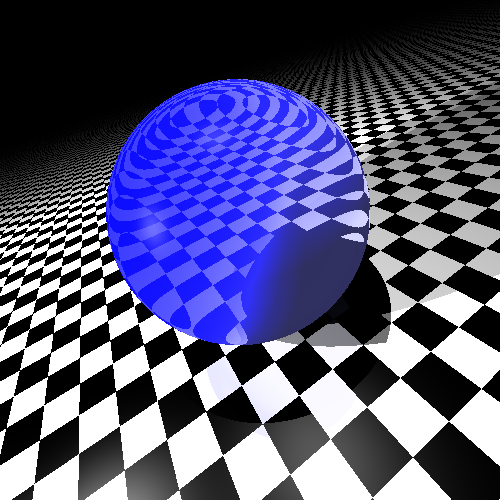
\includegraphics[scale=0.4]{img/transmission.png}
      \caption*{\label{fig:transmission}}
    \end{figure}

  \item 实现了三角面片的渲染,在求交时计算齐次重心坐标,为网格中的法向插值做准备.
    \begin{figure}[H]
      \centering
      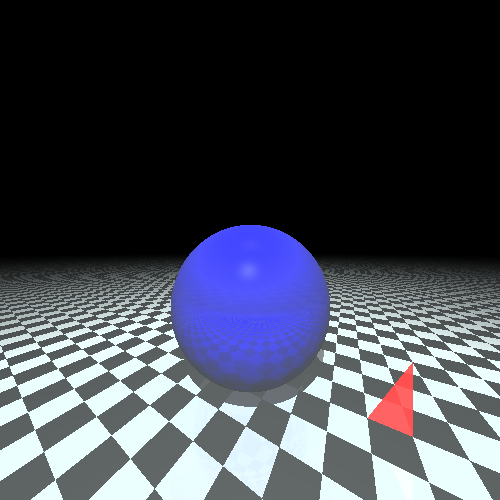
\includegraphics[scale=0.4]{img/face.png}
      \caption*{\label{fig:face}}
    \end{figure}

  \item 实现了obj格式读取及基本的渲染,绘制出了一个红色小人.
    \begin{figure}[H]
      \centering
      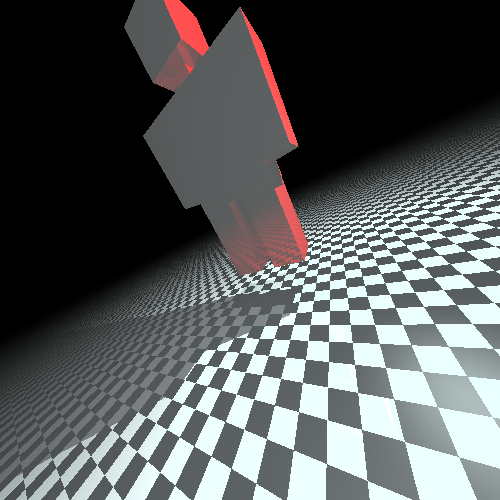
\includegraphics[scale=0.4]{img/human.png}
      \caption*{\label{fig:human}}
    \end{figure}

  \item 实现了KDTree, 可以开始渲染更大的obj.
    \begin{figure}[H]
      \centering
      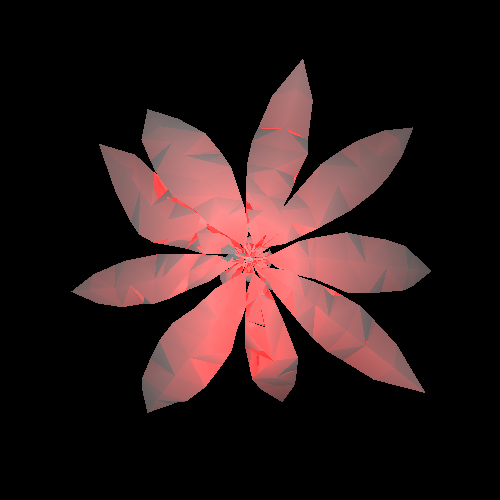
\includegraphics[scale=0.4]{img/flower.png}
      \caption*{\label{fig:flower}}
    \end{figure}

  \item 按照\cite{kdtree}优化了KDTree的实现之后发现如下左图所示bug, 调试很久后发现两个原因.
    一是建树时选取候选切割平面未偏移\verb|EPS|, 二是包围盒求交存在小bug,少了一个绝对值运算.
    其中第二个bug还严重影响了速度,修复后的KDTree相比不用KDTree有了上千倍的速度提升.
    \begin{figure}[H]
      \centering
      \begin{minipage}[b]{0.46\linewidth}
        \centering
        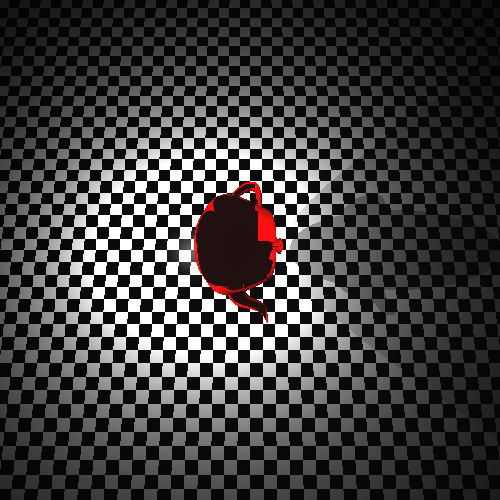
\includegraphics[width=\textwidth]{img/bug_teapot.png}
      \end{minipage}
      \begin{minipage}[b]{0.46\linewidth}
        \centering
        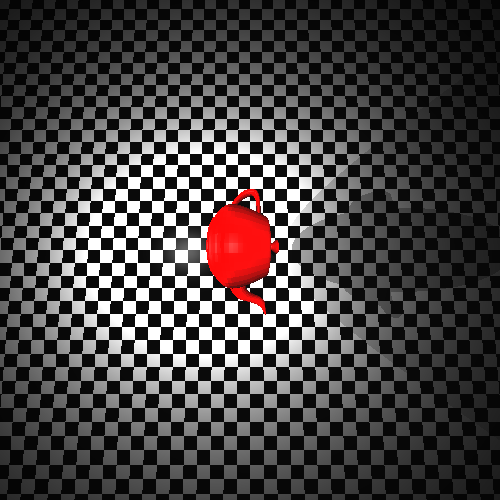
\includegraphics[width=\textwidth]{img/fixed_teapot.png}
      \end{minipage}
      \caption*{\label{fig:kdtree_bug}}
    \end{figure}

  \item 实现了法向量插值,详见\secref{smooth}. 插值前后的效果如下所示:
    \begin{figure}[H]
      \begin{minipage}[b]{0.46\linewidth}
        \centering
        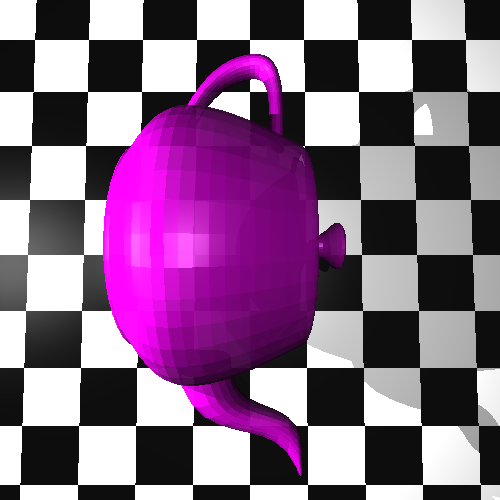
\includegraphics[width=\textwidth]{img/rough.png}
      \end{minipage}
      \begin{minipage}[b]{0.46\linewidth}
        \centering
        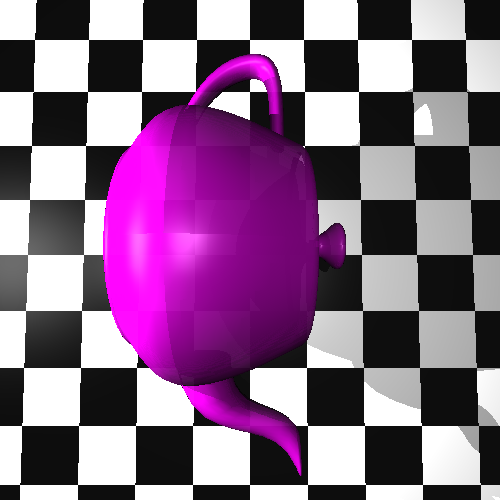
\includegraphics[width=\textwidth]{img/smooth.png}
      \end{minipage}
      \caption{插值的茶壶\label{fig:smooth}}
    \end{figure}

  \item 将KDTree扩展到了整个空间.
    设计方法是将所有的有限大物体合成为一个``KDTree''物体(因为几何物体及KDTree都继承自\verb|Renderable|基类),保留无限大物体,再在
    空间中进行渲染.下图是一个20W面片的龙加上1万个球组成的场景,渲染此图只需1.4s.
    \begin{figure}[H]
      \centering
      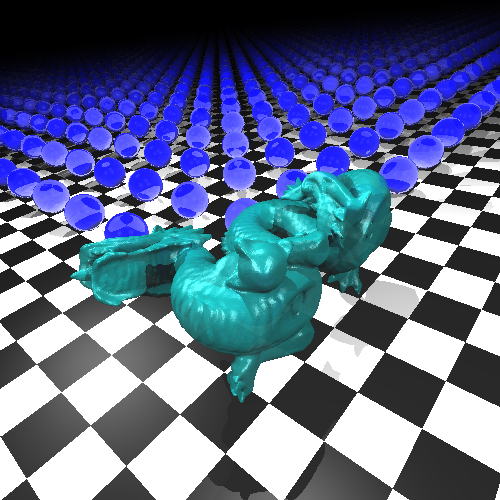
\includegraphics[scale=0.4]{img/dragonball.png}
      \caption*{\label{fig:dragonball}}
    \end{figure}

  \item 加入了图片纹理,设置在平面上.(图中亮斑为点光源所致)
    \begin{figure}[H]
      \centering
      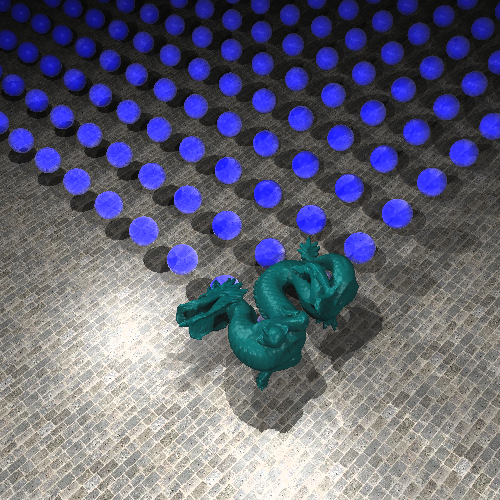
\includegraphics[scale=0.4]{img/pic_texture.png}
      \caption*{\label{fig:texture}}
    \end{figure}

  \item 加入了软阴影效果,详见\secref{soft}.将每个点光源变为20个密集点光源可使左图场景渲染出右图效果.
    左图渲染时间为0.15s, 右图为1.06s
    \begin{figure}[H]
      \begin{minipage}[b]{0.46\linewidth}
        \centering
        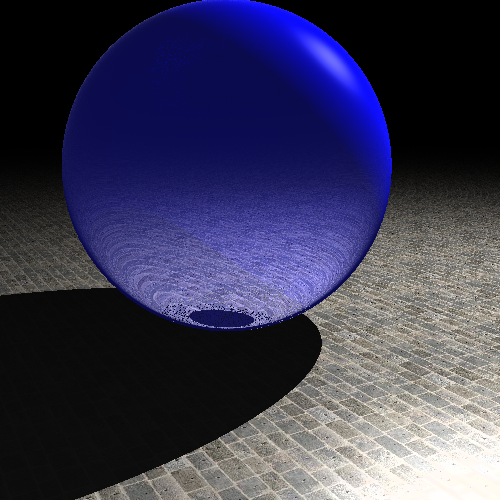
\includegraphics[width=\textwidth]{img/no_soft.png}
      \end{minipage}
      \begin{minipage}[b]{0.46\linewidth}
        \centering
        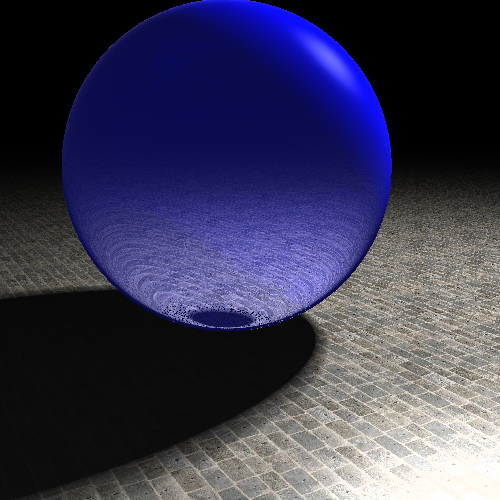
\includegraphics[width=\textwidth]{img/soft.png}
      \end{minipage}
      \caption{软阴影效果图\label{fig:soft}}
    \end{figure}

  \item 加入了抗锯齿效果,能看出变化但效果不明显. 为了图片清晰将此功能关闭.

  \item 发现球与地面接触处有密集的小斑点,调试后发现是由于球底部与平面略微重合,求交时有时会出错.
    \begin{figure}[H]
      \centering
      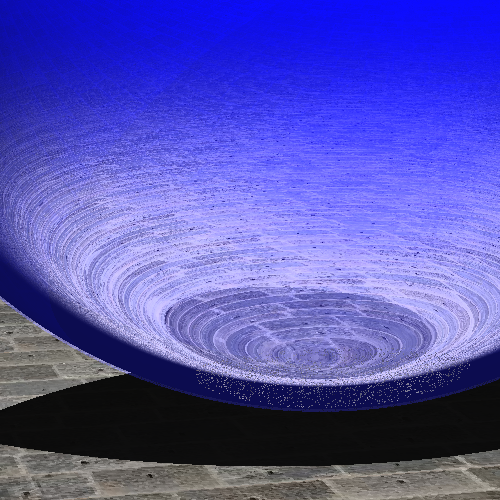
\includegraphics[scale=0.4]{img/smallpoint.png}
    \end{figure}

  \item 加入了景深效果,在感光器处随机取了20个伪视点,效率也相应降低了20倍,效果如图所示.
    \begin{figure}[H]
      \centering
      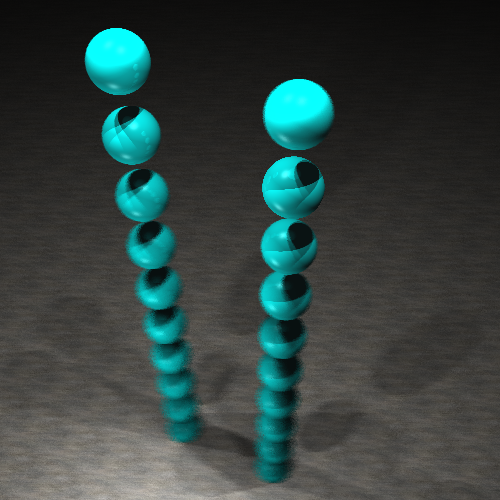
\includegraphics[scale=0.4]{img/dof.png}
      \caption*{\label{fig:dof}}
    \end{figure}

  \item 由于\verb|std::shared_ptr<T>|的默认构造函数会对引用计数和指针对象进行两次内存分配,效率不够高.
    大量换用\verb|std::make_share<T>|后光线追踪时间缩短了40\%.

  \item 利用C++11中的\verb|std::future|实现了KDTree树构建的多线程,建树提速30\%.

  \item 实现了网格简化,并利用堆加速. 对20万面片龙,效果如下.
    \begin{figure}[H]
      \begin{minipage}[b]{0.46\linewidth}
        \centering
        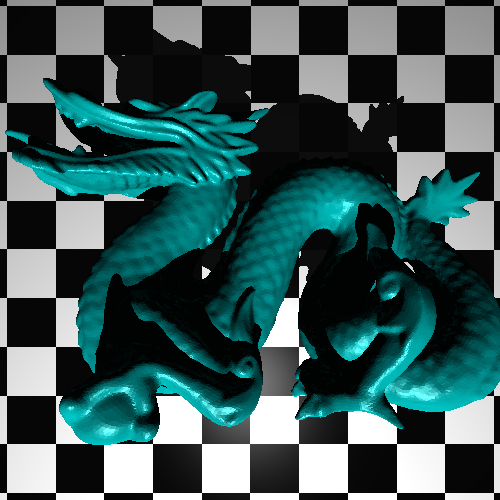
\includegraphics[width=\textwidth]{img/unsimplified_nosmooth.png}
        \caption*{未简化,无法向插值}
      \end{minipage}
      \begin{minipage}[b]{0.46\linewidth}
        \centering
        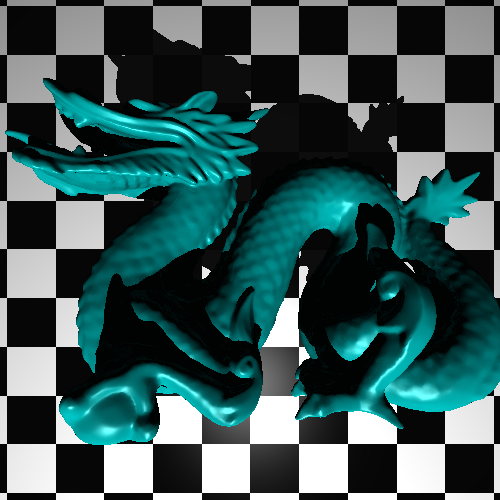
\includegraphics[width=\textwidth]{img/unsimplified_smooth.png}
        \caption*{未简化,含法向插值}
      \end{minipage}

      \begin{minipage}[b]{0.46\linewidth}
        \centering
        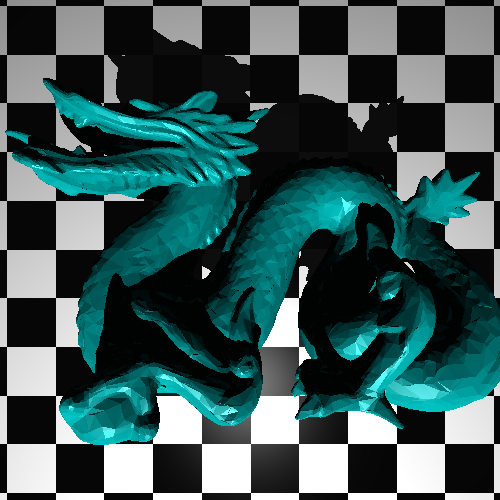
\includegraphics[width=\textwidth]{img/simplified_nosmooth.png}
        \caption*{简化至20\%, 无法向插值}
      \end{minipage}
      \begin{minipage}[b]{0.46\linewidth}
        \centering
        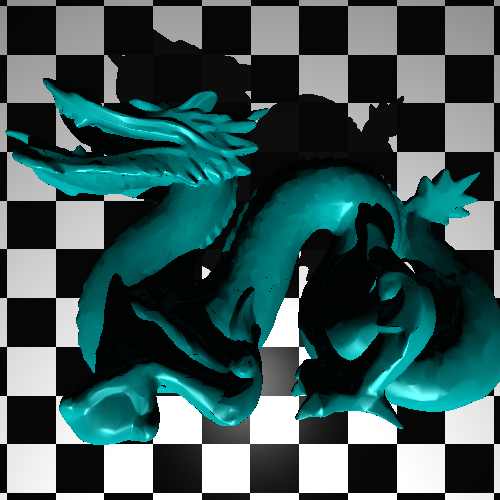
\includegraphics[width=\textwidth]{img/simplified_smooth.png}
        \caption*{简化至20\%, 含法向插值}
      \end{minipage}
      \caption{网格简化效果图\label{fig:simplify}}

    \end{figure}

  \item 发现对于某些模型,简化时会触发\verb|assert|,调试后发现是由于网格坍缩时可能会导致一个面片中三点共线从而无法正确计算出法向.
    将其修正为:若坍缩后面片三点共线,则保留原法向.

  \item 发现在调用\verb|Space::add_obj()|后,若在调用栈中将\verb|Mesh|析构,则会发生段错误.调试后发现是由于
    \verb|Face|类中存储了指向其宿主的指针\verb|Mesh* host|,用于获取插值及纹理信息用,此指针在\verb|Mesh|复制时未被正确更新导致
    得不到其宿主.


  \item 利用Qt4实现了一个简单的GUI,支持单个obj的预览,视点移动,网格简化.

    \begin{figure}[H]
      \centering
      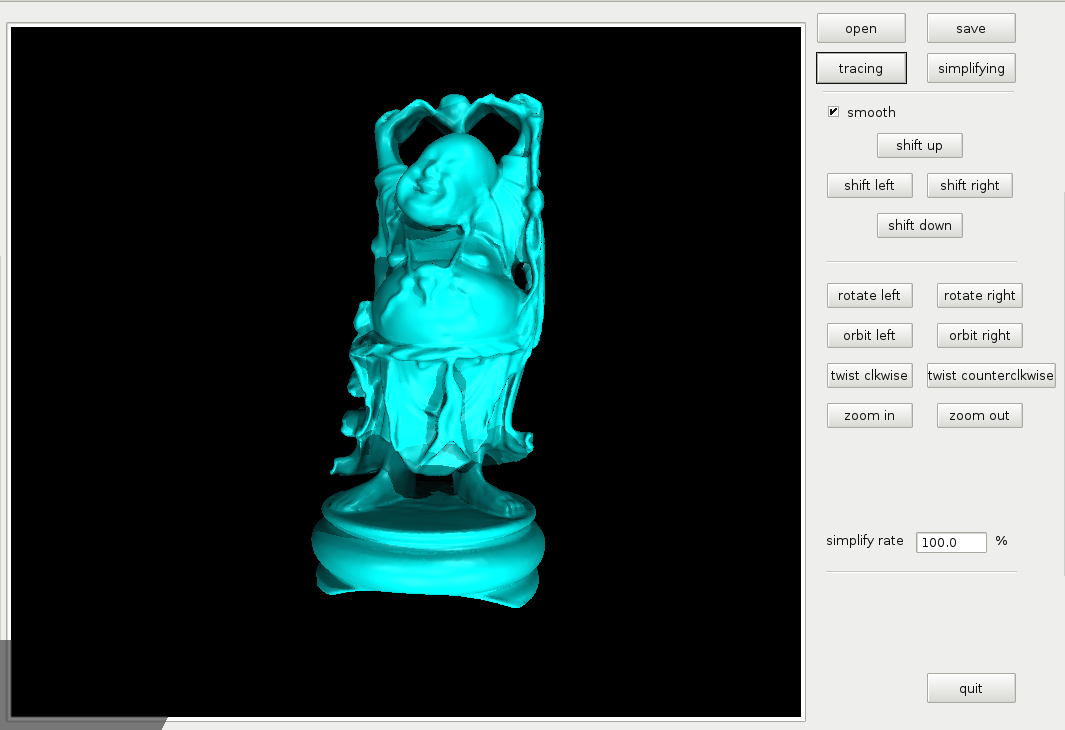
\includegraphics[scale=0.4]{img/gui.png}
      \caption{图形界面展示\label{fig:gui}}
    \end{figure}

  \item 实现了一个简易的全局光照模型,首先按照均匀分布支持了漫反射,渲染效果如下.
    可以看到颜色变化及阴影都更加自然.
    \begin{figure}[H]
      \centering
      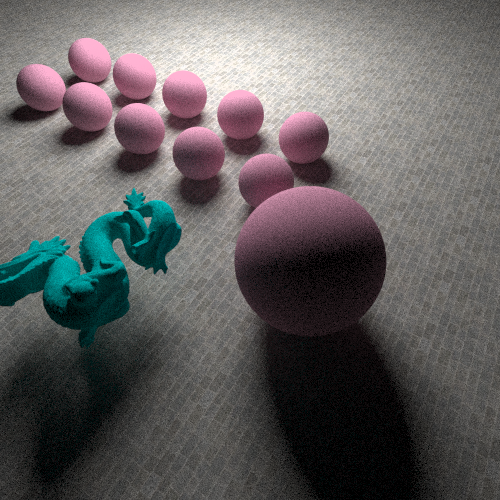
\includegraphics[scale=0.4]{img/gllu_first.png}
    \end{figure}

  \item 为全局光照模型加入了反射效果,若干个镜面的球上可以看到光源的亮斑及互相的反射.
    \begin{figure}[H]
      \centering
      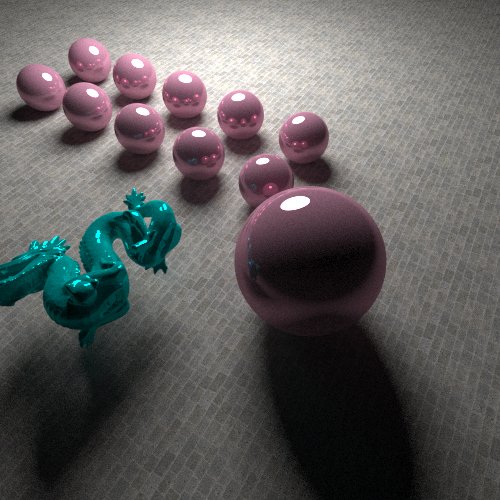
\includegraphics[scale=0.6]{img/gllu_refl.png}
    \end{figure}




\end{enumerate}
